\subsection{Communications}
This section describes the top-level design. Key details can be found in appendix \ref{ap:communications}.

\subsubsection{Selection process}
The selection criteria for a communications protocol were:
\begin{itemize}
	\item The number of devices supported. Systems supporting less than 93 devices were excluded.
	\item Raw data rate. Systems with a raw data rate of less than $\SI{128.32}{\kilo\bit}$ were excluded.
	\item Physical implementation. 
	\begin{itemize}
		\item Connector requirements. Systems with protocol or implementation specific connectors were excluded.
		\item Noise immunity. Systems without in-built noise immunity and error-checking were excluded.
		\item Ease of cabling installation and maintenance. Multi-drop systems were favoured.
		\item Supported topology. Systems that support multiple topologies were preferred.
	\end{itemize}
\end{itemize}

\subsubsection{Master to Daughterboards} 
Given the timing constraints, number of devices and environmental conditions, the evaluation process identified CAN bus and I2C as suitable communications systems.
CAN was chosen primarily due to its differential signalling mechanisms providing inbuilt noise immunity and upper protocol support. 

\subsubsection{CAN Transceiver Selection}
Although the microcontroller has hardware support for the CAN protocol, it does not have the hardware to physically drive the CAN bus lines.
Therefore, a NCV7344 CAN transceiver IC was selected to perform these actions.
It runs off the same $\SI{5}{\volt}$ rail as the microcontroller and is able to withstand the $\SI{105}{\degreeCelsius}$ temperature requirements.

\subsubsection{CAN Bus Physical Implementation}
Separate cabling is used for data communications to meet the timing and signalling requirements of $\SI{1}{\micro\second}$ and $\SI{100}{\micro\second}$.

30-AWG ribbon cable is used for reliability and ease of installation and maintenance.
Using this will mean the bus is not broken if a daughterboard is removed, whilst still meeting the timing requirements.
Additionally, there is a greater range of 10 conductor options (compared to 8, 6 or 4 way) which also provides for dual bus expansion options.
Strain relief is also provided with the chosen connector system.
Figure \ref{fig:data_cable} depicts the arrangement of data signals to provide maximum noise immunity and cable reversal protection.
Note that there are two CAN bus lines that are selectable via a solder jumper on the PCB.
\begin{figure}[H]
	\centering
	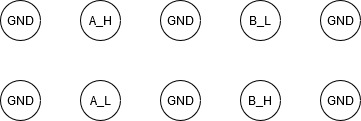
\includegraphics[width=0.4\textwidth]{data_cable}
	\caption{The 10-way data cable with two CAN buses.}
	\label{fig:data_cable}
\end{figure}

\subsubsection{Master to Data Logger}
\textcolor{red}{TODO: Need to do this!!!! Wifi????}
